\documentclass[10pt,twocolumn]{article}

\usepackage[letterpaper,top=0.67in,bottom=0.72in,left=0.67in,right=0.67in,columnsep=0.24in]{geometry}
\usepackage[T1]{fontenc}
\usepackage[utf8]{inputenc}
\usepackage{lmodern}
\usepackage{microtype}
\usepackage{graphicx}
\usepackage{dblfloatfix}
\usepackage{balance}
\usepackage{float}
\usepackage{placeins}
\usepackage{booktabs}
\usepackage{tabularx}
\usepackage{array}
\usepackage{amsmath,amssymb}
\usepackage[numbers,sort&compress]{natbib}
\usepackage[font=small,labelfont=bf,labelsep=period]{caption}
\usepackage{xcolor}
\usepackage{titlesec}
\usepackage{fancyhdr}
\usepackage[hidelinks,breaklinks=true]{hyperref}
\usepackage[nameinlink,noabbrev]{cleveref}

\definecolor{chemblue}{HTML}{26577C}
\definecolor{chemlink}{HTML}{234F70}
\hypersetup{
  unicode=true,
  pdfencoding=auto,
  colorlinks=true,
  linkcolor=chemlink,
  citecolor=chemlink,
  urlcolor=chemlink,
  pdftitle={Executable Chemical Worlds Make Experimental Agency
Measurable},
  pdfauthor={ChemWorld Authors},
  pdfsubject={Executable environments for controlled measurement of AI
experimental behavior},
  pdfkeywords={executable chemical worlds; experimental agency;
autonomous experimentation; AI agents; reproducibility}
}

\setlength{\parindent}{1em}
\setlength{\parskip}{0pt}
\setlength{\emergencystretch}{1.5em}
\setlength{\textfloatsep}{8pt plus 2pt minus 2pt}
\setlength{\floatsep}{7pt plus 2pt minus 2pt}
\setlength{\intextsep}{7pt plus 2pt minus 2pt}
\renewcommand{\dbltopfraction}{0.92}
\renewcommand{\dblfloatpagefraction}{0.75}
\captionsetup{justification=justified,singlelinecheck=false}
% Headings carry their frozen manuscript numbers so the Markdown and TeX
% sources expose the same navigation without duplicate LaTeX counter labels.
\titleformat{\section}{\large\bfseries\color{chemblue}\raggedright\hyphenpenalty=10000\exhyphenpenalty=10000}{}{0pt}{}
\titleformat{\subsection}{\normalsize\bfseries}{}{0pt}{}
\titlespacing*{\section}{0pt}{10pt plus 2pt minus 1pt}{4pt}
\titlespacing*{\subsection}{0pt}{7pt plus 2pt minus 1pt}{3pt}

\pagestyle{fancy}
\fancyhf{}
\fancyhead[L]{\footnotesize Executable Chemical Worlds}
\fancyhead[R]{\footnotesize arXiv preprint}
\fancyfoot[C]{\thepage}
\renewcommand{\headrulewidth}{0.25pt}

\newcommand{\code}[1]{\texttt{#1}}
\providecommand{\tightlist}{%
  \setlength{\itemsep}{0pt}\setlength{\parskip}{0pt}}

\title{\vspace{-1.8em}\textbf{Executable Chemical Worlds
Make\\Experimental Agency Measurable}}
\author{%
ChemWorld Authors%
%
%
}
\date{}

\begin{document}

\twocolumn[
\begin{@twocolumnfalse}
\maketitle
\begin{abstract}
Scientific agents are commonly judged by the best condition they report,
but that endpoint cannot reveal the experimental policy that produced
it. We present ChemWorld, an executable chemical-world apparatus that
makes experimental agency observable. Agents choose typed state-changing
operations, measurements, resource expenditure, termination, final assay
and discard; every accepted transition is identity-bound and exactly
replayable. Compiled controls comprising 29,580 simulator executions
across two task families separate outcome, held-out prediction,
calibration and claim reliability. Two independently configured
primitive-control systems then closed 120 batch lifecycles in five
matched worlds. Codex requested 60 final assays and no discards;
DeepSeek V4 Flash requested 24 final assays and explicitly discarded 36
batches, despite nearly identical non-final instrument use. Fresh Codex
sessions in two deliberately selected worlds yielded eight complete
matched information-condition pairs. Best-of-campaign and raw terminal
contrasts were directionally discordant in two pairs, while full
trajectories separately resolved discovery, retention, drawdown and
recovery. These results establish experimental agency as a measurable
profile of decisions and trajectories, rather than a score recoverable
from the endpoint alone.
\end{abstract}
\vspace{0.6em}
\end{@twocolumnfalse}
]

\section{1. Introduction}\label{introduction}

When a scientific agent reports a high-performing condition, the most
important question is no longer only \emph{what score did it obtain?} It
is also \emph{what kind of experimental process produced that score?} A
condition may be found early and retained, found once and abandoned,
recovered after a drawdown, or reached at the end of an otherwise
uninformative search. These trajectories imply different capabilities
even when their final values agree.

This distinction is difficult to measure with existing evaluation
regimes. Prediction benchmarks remove the act of experimentation.
Optimization benchmarks expose a value-returning oracle but usually
collapse each experiment to a vector query. Self-driving laboratories
and instrument-operating agents provide indispensable evidence about
physical execution, automation and deployment
\citep{szymanski2023alab, dai2024mobile, darvish2025organa, vriza2026instruments},
but a physical apparatus cannot usually be cloned many times while
changing only the information supplied to the agent. As a result, the
agent's experimental behavior is often entangled with a particular
laboratory, material batch and observation history.

ChemWorld fills this measurement gap with executable chemical and
chemical-engineering worlds. The central design choice is simple:
\textbf{the agent is the experimental subject; the chemical world is the
apparatus}. Within a stateful, partially observable world, the agent
selects additions, process conditions, measurements, termination and
final assay. The environment records the consequence of every choice,
including invalid operations, failed attempts and resource use. Matched
hidden-world identities permit controlled information contrasts, while
fresh sessions in the same physical world measure behavioral
repeatability.

This apparatus changes what can be asked of a scientific agent. Instead
of reducing performance to one leaderboard value, we can measure
lifecycle completion, within-campaign best-discovery position, retention
of an incumbent, drawdown, recovery, terminal quality, prediction and
claim reliability. These are operational readouts of behavior, not
inferred mental states. Their non-equivalence is itself a scientific
result: similar endpoint outcomes can arise from different experimental
histories and capabilities.

We use three evidence layers. First, compiled experiments compare
matched material-information conditions across two task families and
separate optimization from prediction, calibration and claim
reliability. Second, primitive-control campaigns show that distinct
complete agent systems can close experimental lifecycles under a shared
resource ledger while expressing different assay and discard policies.
Third, fresh trajectories in matched physical worlds reveal which
behavioral features recur and which vary between sessions. Together they
establish the paper's central result: \textbf{an experimental endpoint
is an incomplete readout of experimental agency}.

Our contributions are:

\begin{enumerate}
\def\labelenumi{\arabic{enumi}.}
\tightlist
\item
  an executable, chemistry-native apparatus with stateful operations,
  active measurements, failures, resource accounting, identity control
  and exact physical replay;
\item
  a primitive-control protocol, exercised by two complete agent systems,
  in which the agent---rather than a fixed recipe---chooses operations,
  observations, assay commitment and lifecycle termination;
\item
  matched information conditions and fresh sessions that make endpoint
  optimization, prediction, claims, discovery, retention, drawdown and
  recovery separately observable; and
\item
  empirical evidence that the endpoint underdetermines the process: raw
  terminal performance can change opposite to best-of-campaign
  performance, while full trajectories expose experimental policies that
  neither scalar records.
\end{enumerate}

\section{2. Relation to existing
systems}\label{relation-to-existing-systems}

Self-driving laboratories optimize reactions and materials in real
hardware, and chemistry agents increasingly connect language models to
literature, planning tools and robotic execution
\citep{boiko2023autonomous, bran2024augmenting, panapitiya2026autolabs, pilon2026robochemflex}.
Their defining strength is physical validity: they answer whether a
proposed workflow can be executed and whether automation can operate
reliably. ChemWorld addresses a complementary question---whether the
experimenting agent can be isolated, intervened on and repeated under
matched physical identity.

Digital optimization suites provide controlled objective functions and
scalable algorithm comparison \citep{felton2021summit, hase2021olympus}.
Interactive science environments extend this idea toward stateful
control, discovery and model identification
\citep{beeler2024chemgymrl, bloor2024pcgym, jansen2024discoveryworld, gandhi2025boxinggym, duan2025scigym, nagele2026sciexplorer}.
ChemWorld's distinctive unit is a chemical experiment as a
resource-consuming sequence of typed operations and measurements, not a
single parameter query. The same world can be replayed under different
information and authority conditions without changing its hidden
physical identity.

Recent work treats agents themselves as behavioral objects and studies
how environment design changes scientific discovery
\citep{chen2026agentbehavior, xin2026eurekagent, riosgarcia2026scientifically}.
ChemWorld brings that perspective to chemistry-native experimental
lifecycles. Its contribution is the combination of matched chemical
worlds, primitive action authority, evidence access, campaign-wide
resources, immutable trajectories and within-world fresh-session
replication. It does not replace a robotic laboratory; it provides the
controlled measurement apparatus that a real laboratory cannot
economically instantiate at scale.

\section{3. ChemWorld makes experimental agency
measurable}\label{chemworld-makes-experimental-agency-measurable}

\subsection{3.1 Executable worlds rather than value-returning
oracles}\label{executable-worlds-rather-than-value-returning-oracles}

A ChemWorld task defines a hidden physical state, public observation
contract, typed operations, instrument responses, resource endowment,
failure semantics and one or more evaluator-bound endpoints. Operations
change state. Measurements are actions with costs and timing
consequences. Termination closes a vessel, and a final assay is
explicitly requested rather than automatically revealed.

The qualified environment surface contains 15 registered tasks, 28
operation types, five instrument classes, 415 deterministic
complete-experiment boundary cases and 62 evaluator-bound endpoints
(Fig. 1). Qualification establishes runtime reachability and evaluator
binding. The empirical paper uses two tasks for compiled controls and
one for autonomous primitive control, keeping platform scope and
evidence scope explicit.

\begin{figure*}[!tbp]
\centering
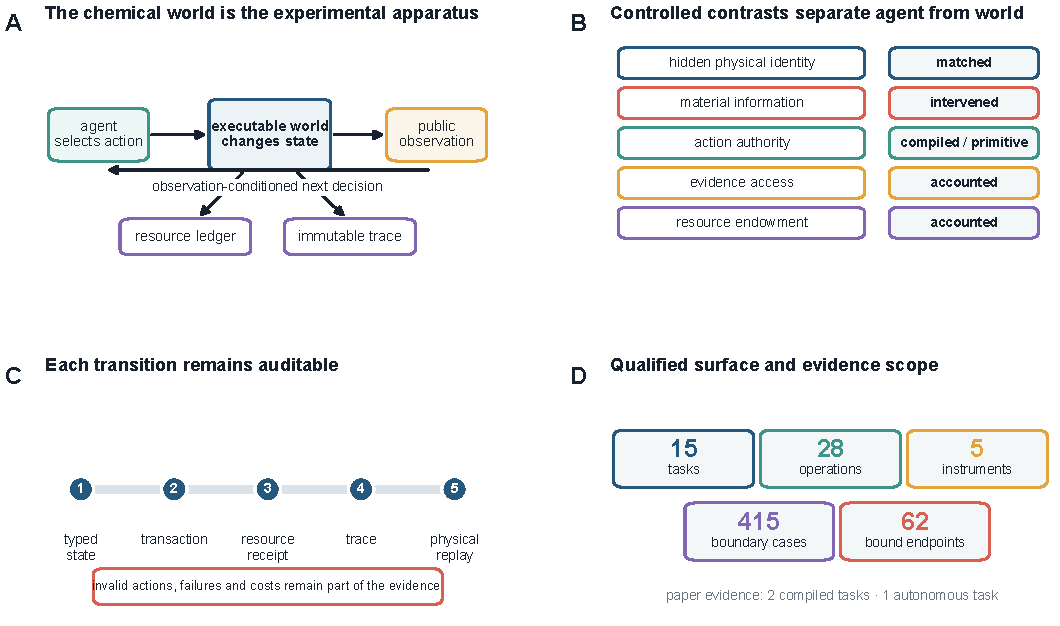
\includegraphics[width=\textwidth]{figures/figure-1-controlled-apparatus.pdf}
\caption{\textbf{ChemWorld is a controlled apparatus for measuring experimental agency.}
\textbf{A,} The agent selects a typed action, the executable world changes state, and only the public observation returns to the agent; the transition also writes a resource ledger and immutable trace.
\textbf{B,} Physical identity and material information can be matched or intervened on while authority, evidence and resources remain explicit parts of the protocol.
\textbf{C,} Typed state, transactions, receipts, traces and physical replay form an auditable spine; invalid actions and failures remain evidence.
\textbf{D,} Qualified platform surface and the narrower evidence scope used in this paper.}
\label{fig:apparatus}
\end{figure*}

\subsection{3.2 Controlled identity, resources and
replay}\label{controlled-identity-resources-and-replay}

Every run binds source, configuration, task, physical world, material
instance, observation namespace and trajectory identity. The public
agent view excludes hidden evaluator state. Accepted operations are
transactional: a successful transition updates state and consumes the
corresponding resources; a rejected operation records its failure
without silently repairing the action.

The campaign ledger spans raw materials, solvent, vessels, non-final
instrument uses, operation attempts and provider sessions. This design
makes opportunity cost part of the experimental record while keeping the
ledger external to the prompt. Agents access compact status and history
artifacts on demand rather than receiving a continually expanding
transcript.

Exact replay means exact reconstruction of environment transitions,
public observations and resource changes from the stored trajectory. It
does not mean regeneration of the language model's token sequence.
Fresh-session replication therefore deliberately samples a new agent
trajectory while holding the physical world fixed.

\subsection{3.3 Evidence layers and analysis
units}\label{evidence-layers-and-analysis-units}

The number of executed world transitions measures use of the apparatus,
not the number of statistically independent samples. Table 1 separates
those quantities throughout the paper.

\begin{table*}[t]
\centering
\caption{\textbf{Evidence layers and effective analysis units.} Execution counts describe the scale at which the apparatus was exercised; inference is organized around worlds and fresh session-level pairs.}
\label{tab:evidence}
\small
\begin{tabularx}{\textwidth}{@{}p{0.18\textwidth}p{0.25\textwidth}p{0.20\textwidth}X@{}}
\toprule
Evidence layer & Purpose & Executions & Primary analysis unit \\
\midrule
Platform qualification & Reachability and evaluator binding & 415 boundary cases & declared task/endpoint \\
Compiled control & Task, information and diagnostic calibration & 29,580 simulator executions & paired physical world; 10 per task and arm \\
Primitive-control systems & Lifecycle autonomy, interface portability and trajectory policy & 120 closed vessels; 1,704 operations & complete agent system by world and arm; 2 systems, 5 worlds \\
Fresh-session replication & Within-world directional repeatability & 114 started vessels; 112 final assays & world by session-level arm pair; 4 complete pairs per world \\
\bottomrule
\end{tabularx}
\end{table*}

\section{4. Compiled controls separate outcome from evidence
use}\label{compiled-controls-separate-outcome-from-evidence-use}

Compiled control gives the agent a bounded complete-experiment
interface. It is not the target autonomy setting; it is a controlled
calibration that can be run across tasks, information conditions and
classical optimization policies.

Across ten sequentially collected matched worlds, the
nominal-information arm produced a mean nominal-minus-opaque score
difference of 0.072 in electrochemical conversion (8/10 positive worlds;
97.5\% per-task world-bootstrap interval 0.007 to 0.155) and 0.026 in
reaction-to-crystallization (7/10 positive; interval -0.013 to 0.063).
The two 97.5\% intervals are multiplicity-adjusted descriptive stability
intervals for the pre-specified two-task analysis. Thus the matched
information conditions were associated with distinct outcome profiles in
the two executable task families (Fig. 2A).

The deliberately misindexed arm provides a manipulation check. It
redirected the first material-sensitive action in 70\% of
electrochemical worlds and 100\% of crystallization worlds.
Misleading-action share subsequently fell from 0.54 to 0.24 in
electrochemistry and from 0.86 to 0.50 in crystallization (Fig. 2B). The
distinction among action manipulation, later correction and performance
restoration is important: both tasks passed the behavior-change check,
while their correction and score-restoration checks differed, and
neither passed the joint rule (Fig. 2C).

Outcome and epistemic diagnostics also gave different profiles. In the
opaque arm, electrochemical conversion combined a 0.715 endpoint score
with 0.744 held-out directional accuracy, a 0.186 Brier score and a
0.611 unsupported-claim rate. Reaction-to-crystallization yielded 0.535,
0.478, 0.298 and 0.714, respectively. These measurements are reported
separately because none is a substitute for another (Fig. 2D).

\begin{figure*}[!tbp]
\centering
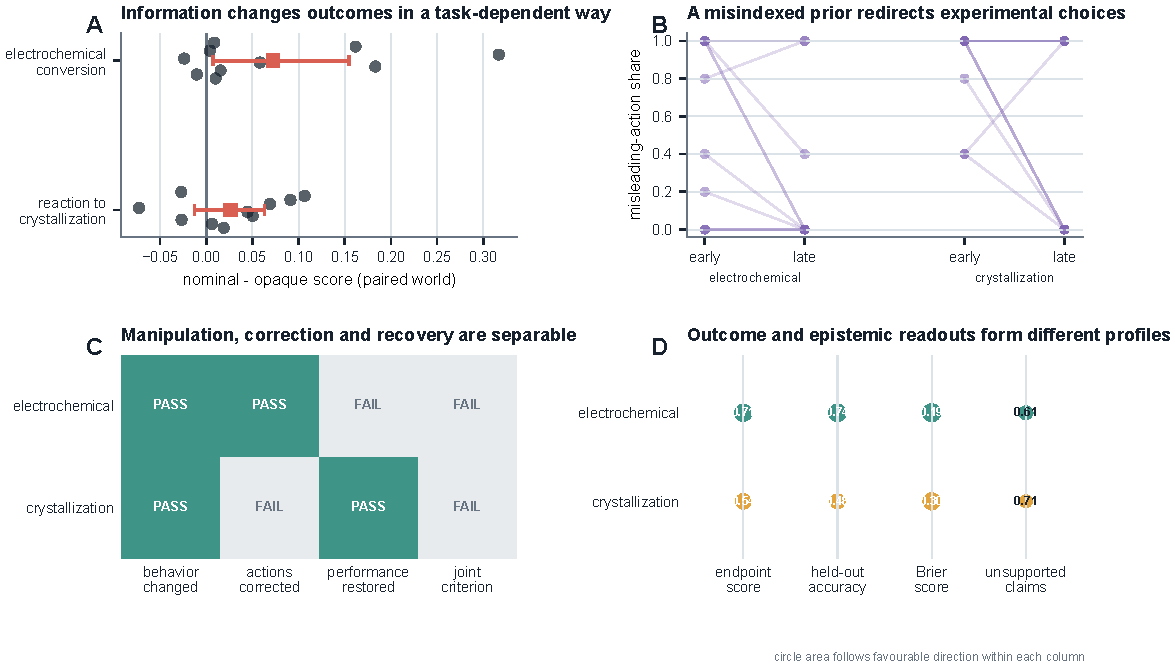
\includegraphics[width=\textwidth]{figures/figure-2-compiled-controls.pdf}
\caption{\textbf{Compiled controls distinguish task outcome, information response and epistemic readouts.}
\textbf{A,} Paired nominal-minus-opaque score differences across ten worlds per task; squares show means and multiplicity-adjusted 97.5\% per-task world-bootstrap stability intervals.
\textbf{B,} World-level early-to-late misleading-action shares under a deliberately misindexed material prior.
\textbf{C,} Commit-frozen manipulation, correction, performance-restoration and joint criteria.
\textbf{D,} Raw task-level endpoint, held-out prediction, calibration and unsupported-claim readouts. Circle area follows the favourable direction within each metric column; the printed number is the raw value.}
\label{fig:compiled}
\end{figure*}

Classical optimizers are retained as calibration controls rather than
the paper's target competition. Complete world-level contrasts for every
baseline, including exact sign summaries and leave-one-world-out ranges,
are provided in the sensitivity artifact. This keeps the empirical
question aligned with the paper's contribution: what aspects of
experimental behavior become measurable once the world is a controlled
apparatus?

\section{5. One apparatus resolves distinct autonomous experimental
policies}\label{one-apparatus-resolves-distinct-autonomous-experimental-policies}

We exercised the primitive-control protocol with two complete agent
systems on the same five physical worlds and two material-information
arms. Both received the same typed action space, instrument access,
campaign resource card, hidden world and material identities,
observation noise and scoring contract. Native Codex
(\texttt{gpt-5.6-sol}, medium reasoning) acted through a fresh MCP
session for each vessel. DeepSeek V4 Flash made one schema-validated
JSON decision per primitive operation through a direct provider loop.
Because model and scaffold change together, this is not an isolated
backend comparison. It asks a more basic apparatus question: can
distinct autonomous systems inhabit the same experimental world and
leave comparable, auditable behavioral traces?

Both systems passed that test. Each closed all six batch opportunities
in all ten cells, yielding 120 closed lifecycles under matched physical
identity (Fig. 6). Their closure policies were sharply different. Codex
requested a final assay for all 60 batches and discarded none. DeepSeek
requested 24 final assays and explicitly discarded 36 batches. Yet their
use of non-final instruments was nearly identical (164 versus 163),
while their operation totals were 815 and 889. Thus a scalar completion
flag would call both systems identical, and a score-only view would omit
36 deliberate abandonment decisions. The executable apparatus instead
separates evidence acquisition, continued investment, terminal assay
commitment and discard.

Material information also altered these policies within the DeepSeek
system. Across the five nominal-information cells it committed 16
batches to final assay and discarded 14; under opaque codes it committed
eight and discarded 22. The nominal arm additionally used 67 more
primitive operations. Codex committed all 30 batches in each arm to
final assay. With five paired worlds these are descriptive
system-specific profiles, not a population estimate, but they show that
a material-information contrast can be expressed through resource and
lifecycle decisions rather than endpoint score alone.

Figure 3 reconstructs the Codex implementation, for which each vessel
received a public workspace and typed tools while the complete ledger
remained external to the prompt. Figure 3A shows one vessel. The
important feature is not the particular seven-operation sequence; it is
the placement of observation before the next agent decision. A
UV--visible measurement entered public state before the agent chose to
terminate and request the final assay. Figure 3B shows this lifecycle
across every Codex vessel and information arm, while Fig. 3C
reconstructs its campaign-level resource receipt.

\begin{figure*}[!tbp]
\centering
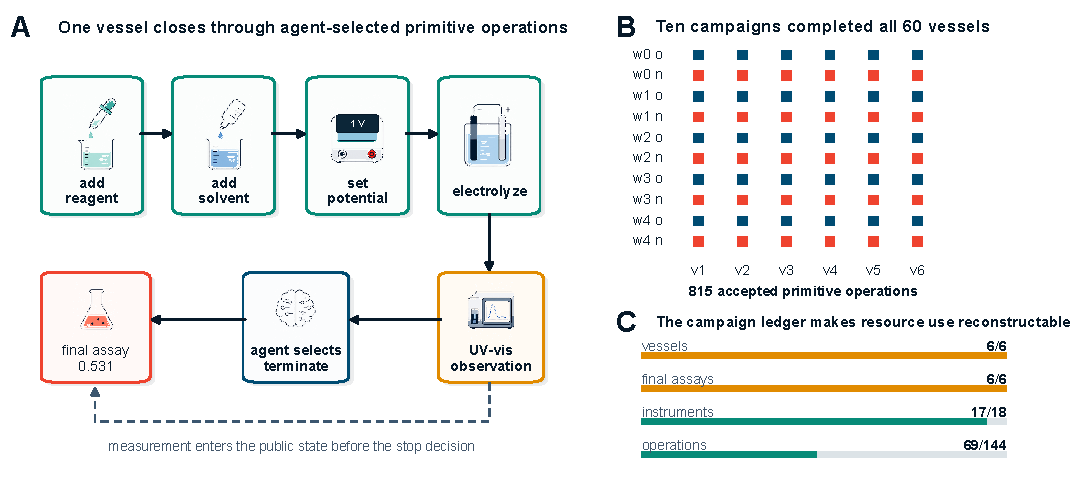
\includegraphics[width=\textwidth]{figures/figure-3-autonomous-lifecycle.pdf}
\caption{\textbf{A primitive-control agent closes complete experimental lifecycles.}
\textbf{A,} One seven-operation vessel in which a UV--visible observation is available before agent-selected termination and explicit final assay.
\textbf{B,} All six Codex vessels reached final assay in each of ten world-by-information campaigns; navy denotes opaque codes and coral denotes nominal properties.
\textbf{C,} The immutable trajectory reconstructs the campaign resource receipt. The example is descriptive and is not part of the fresh-session replication estimand.}
\label{fig:autonomy}
\end{figure*}

\section{6. Endpoint scores conceal experimental
trajectories}\label{endpoint-scores-conceal-experimental-trajectories}

The six-assay Codex campaigns expose structure that a final
recommendation cannot contain. Figure 4 follows six final assays in
three development worlds. In world 0, the opaque trajectory lost its
initial score, recovered by the fourth assay and finished near the
nominal trajectory. In world 2, the opaque arm discovered its campaign
best immediately and then lost it, whereas the nominal arm improved and
retained a higher terminal value. In world 4, both arms began similarly
but their terminal behavior diverged sharply.

We operationalize these patterns with four lifecycle readouts.
Within-campaign best-discovery position records when the observed
campaign maximum first appears. Online retention asks whether a new
assay remains within a pre-specified fraction of the pre-assay
incumbent. Maximum absolute drawdown records the largest departure from
that incumbent. Terminal-to-best ratio records how much of the observed
campaign best remains at the final assay. Loss episodes and recovery
delays provide additional summaries when a trajectory falls below its
retention boundary.

\begin{figure*}[!tbp]
\centering
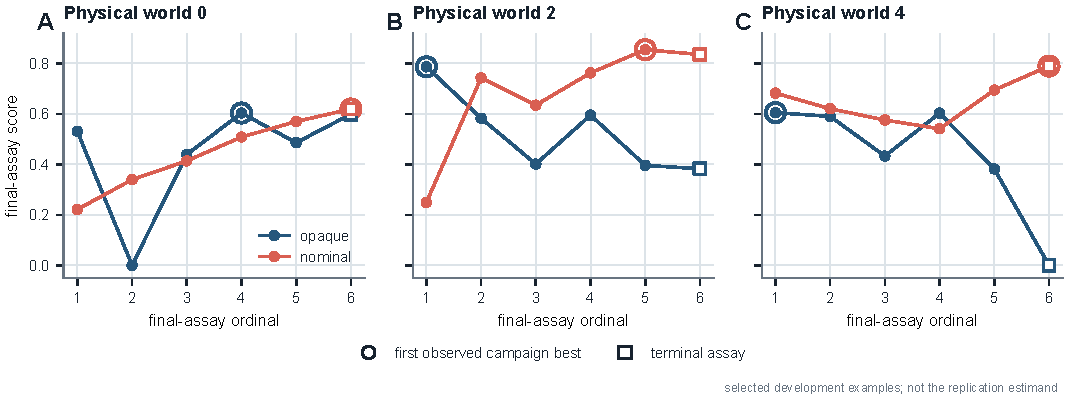
\includegraphics[width=\textwidth]{figures/figure-4-trajectory-dynamics.pdf}
\caption{\textbf{Similar endpoints can arise from different experimental trajectories.}
Selected development worlds illustrate early discovery followed by loss, gradual improvement, retention and terminal divergence. Open circles mark the first observed campaign best; squares mark terminal assays. Navy denotes opaque material codes and coral denotes nominal material properties. These examples motivate the lifecycle readouts but are not the replication estimand.}
\label{fig:trajectories}
\end{figure*}

Across the five development worlds, nominal information was associated
with later within-campaign best discovery on average (0.80 versus 0.32
of the six-assay horizon), together with higher retention (0.72 versus
0.52), smaller mean maximum drawdown (0.092 versus 0.333), greater
pooled recovery (0.80 versus 0.50) and higher terminal-to-best ratio
(0.941 versus 0.671). Because each arm contains one session per
development world, these values describe the five matched demonstration
worlds. Their role is to show what the apparatus resolves: best
discovery, retention, drawdown, recovery and relative terminal retention
are simultaneously observable coordinates of a trajectory, none of which
is recorded by the best score alone.

\section{7. Fresh sessions test within-world
repeatability}\label{fresh-sessions-test-within-world-repeatability}

We selected physical worlds 1 and 3 before the replication launch
because their development contrasts pointed in different directions. The
commit-frozen design crossed two worlds, five fresh trajectory
replicates and two information arms. Each cell received six vessel
opportunities and the same physical, observation and resource identities
as its within-replicate counterpart; the provider did not expose a
controllable sampling seed.

Eighteen of 20 cells completed. Two cells were right-censored after 50
and 56 accepted operations by provider-infrastructure failures, leaving
four complete pairs in each world. All ten planned pairs remain visible
in Fig. 5. The 75\% classification rule was frozen after launch while
endpoint and lifecycle outcomes remained uninspected; it classified a
world-by-metric result as directional when at least three of four
available differences shared a sign and the median shared that
direction.

The authoritative matrix followed a launcher-level restart after an
infrastructure incident in the first launch; the restart decision was
recorded before outcome inspection. The protocol deviation, excluded
trajectories and separate sensitivity check are reported in Methods
10.7.

The continuous pairwise data provide an algebraically independent
endpoint check. Across the eight complete pairs, nominal-minus-opaque
best-of-campaign and raw terminal contrasts were sign-discordant in two
pairs; their descriptive Pearson correlation was \(+0.826\). The
clearest instance was world 3/r01: the best-score contrast was
\(-0.167\), whereas the raw terminal contrast was \(+0.240\). Thus even
strongly co-varying endpoint summaries are not interchangeable for an
individual experimental trajectory.

Full process profiles expose substantially more structure (Fig. 5B).
Each complete pair has separate signed contrasts for best score, raw
terminal score, discovery timing, online retention, drawdown and
relative terminal retention. The frozen 75\% classification summarized
six of eight selected world-by-lifecycle cells as mixed. That
categorical count is supporting rather than the main result: across the
complete threshold-by-zero-handling grid it ranges from two to eight,
whereas the continuous contrasts and both right-censored pairs remain
visible without thresholding. The terminal-to-best ratio is retained as
a relative-retention readout; because it reuses the best score in its
denominator, it is not treated as algebraically independent of the
best-score contrast.

\begin{figure*}[!tbp]
\centering
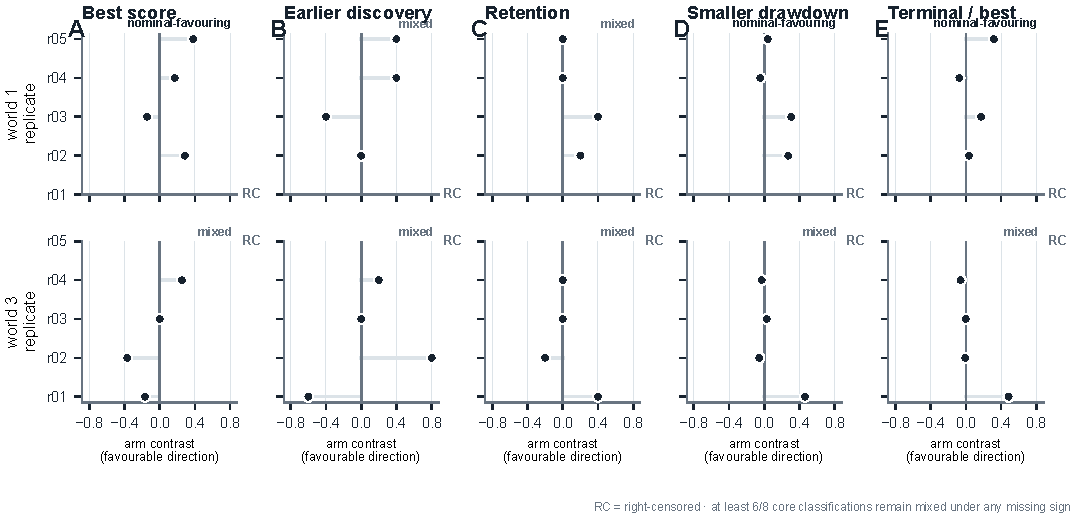
\includegraphics[width=\textwidth]{figures/figure-5-within-world-replication.pdf}
\caption{\textbf{Fresh trajectories expose information that endpoint summaries omit.}
\textbf{A,} Each point is one complete fresh-session pair in a fixed physical world. Shaded quadrants mark opposite signs for best-of-campaign and raw terminal score; two of eight pairs occupy them. Labels identify trajectory replicates, not shared model randomness.
\textbf{B,} Continuous nominal-minus-opaque contrasts for all ten planned pairs. Positive values favour nominal information after orienting discovery and drawdown to their favourable directions; grey rows are right-censored. Relative retention is shown as a supporting process readout, not an endpoint-independent contrast.}
\label{fig:replication}
\end{figure*}

The fresh sessions therefore expose two forms of information that a best
score cannot contain: raw terminal disagreement within a matched pair
and trajectory-to-trajectory variation across the complete process
profile. Both become directly observable because world identity,
observation stream, resource card and action authority remain
controlled.

\section{8. Experimental agency is a profile, not a
scalar}\label{experimental-agency-is-a-profile-not-a-scalar}

The compiled and primitive-control studies measure complementary parts
of experimental agency. Compiled control separates task outcome from
prediction, calibration and claim diagnostics. Primitive control
additionally reveals what a system does with its experimental
opportunities. Figure 6 makes that distinction concrete for two complete
agent systems under the same matched apparatus.

\begin{figure*}[!tbp]
\centering
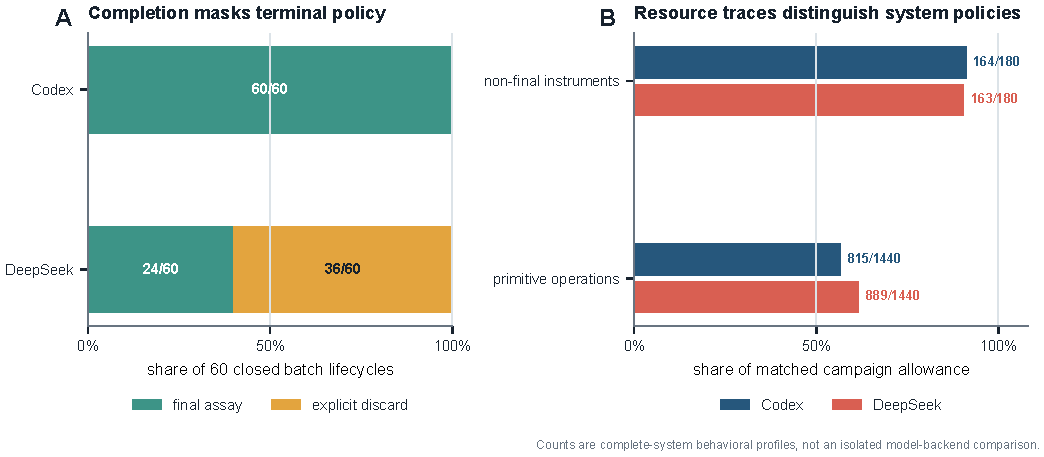
\includegraphics[width=\textwidth]{figures/figure-6-experimental-agency-profile.pdf}
\caption{\textbf{Lifecycle completion does not specify experimental policy.}
\textbf{A,} Both complete agent systems closed all 60 matched batch lifecycles, but Codex committed every batch to final assay whereas DeepSeek V4 Flash explicitly discarded 36.
\textbf{B,} Their non-final instrument use was nearly identical, while their primitive-operation use and terminal policies differed. Fractions use the common ten-campaign allowances. These are complete-system behavioral profiles, not an isolated model-backend comparison.}
\label{fig:profile}
\end{figure*}

The profile view supports a stronger evaluation standard for scientific
agents. Lifecycle closure, evidence acquisition, continued investment,
assay commitment, discard, retention and recovery are distinct
observables. ChemWorld provides a common apparatus that measures them
separately and preserves the decisions from which each readout is
computed.

\section{9. Discussion}\label{discussion}

ChemWorld contributes a new experimental object: the process by which an
agent experiments. Its value does not depend on replacing a self-driving
laboratory or winning a universal optimization leaderboard. It occupies
a different and useful role. A real laboratory establishes physical
executability; an optimization suite calibrates search; an executable
chemical world can clone physical identity, intervene on information and
authority, preserve failures, and sample fresh decision trajectories at
low marginal cost.

The present experiments demonstrate four consequences. First, matched
information conditions are associated with different actions, endpoint
outcome, prediction and claim reliability profiles. Second, two complete
agent systems can close the same matched batch lifecycles while
allocating terminal assays and discards very differently; the apparatus
therefore measures experimental policy rather than merely interface
compliance. Third, autonomous lifecycle completion does not specify how
a high-performing condition was discovered, retained or recovered.
Fourth, best-score and raw terminal contrasts can reverse sign within
matched fresh sessions, while the full process profiles separate
additional dimensions that neither endpoint records. The resulting
conclusion is operational and direct: best-of-campaign performance
underdetermines the experimental process that produced it.

The same apparatus makes a broader class of controlled studies possible.
World mechanisms, observation channels, material semantics, instruments,
resource endowments and failure laws are executable components rather
than constraints imposed by one physical laboratory. They can therefore
be recombined while agent authority and audit semantics remain fixed.
This programmability is what turns experimental agency from an anecdotal
trace into a scalable object of study.

The second agent system supplies an initial interface-portability
demonstration, not a general agent ranking. The next scientific use of
this apparatus is a factorial measurement program: randomly sampled
worlds, multiple mechanism families, multiple complete agent systems,
controlled evidence access and matched resource endowments. Such
experiments can estimate world heterogeneity, trajectory variability and
intervention response hierarchically, and can test whether lifecycle
reliability predicts transfer, recovery from misinformation or behavior
under scarcity.

Synthetic instruments and scoring laws make those interventions
inexpensive and repeatable. A calibrated physical or high-fidelity
bridge can then test which trajectory phenomena transfer to a particular
laboratory system. The two forms of evidence are complementary:
executable worlds identify controlled behavioral structure; physical
laboratories establish deployment validity.

\FloatBarrier

\section{10. Methods}\label{methods}

\subsection{10.1 Environment
qualification}\label{environment-qualification}

The task registry and runtime-domain audit declare task contracts, typed
operations, instrument interfaces, state invariants and evaluator-bound
success metrics. Qualification required deterministic reachability
through 415 complete boundary cases and binding of all 62 declared
endpoints to evaluator state. The qualified surface contains 15 tasks,
28 operation types and five instruments. These counts characterize
supported environment capabilities; empirical agent results are reported
only for the task families actually exercised.

\subsection{10.2 Compiled-control
protocol}\label{compiled-control-protocol}

Compiled control covered electrochemical conversion and
reaction-to-crystallization. Each task used physical world seeds 0--9
and three information conditions: opaque material codes, anonymous
nominal properties and a commit-frozen misindexed prior. Each
participant session selected 20 complete experiments, after which a
replay verifier recomputed all scores from the immutable reports.
Classical policies used the same world identities, budgets and
information contracts.

The opaque condition replaced material identities by stable anonymous
codes. The nominal condition exposed the correct anonymous
material-family property rows without revealing latent world residuals.
The misindexed condition transposed one targeted material row chosen
using independent qualification worlds before the formal campaigns; the
affected mapping was fixed across the ten formal worlds. These
conditions therefore modify the supplied prior while holding the
physical world, action space, score and budget fixed. Opaque, nominal
and misindexed campaigns entered the release as sequential commit-frozen
extensions that reused the earlier matched cells. We therefore report
matched-world associations and do not use execution order as a causal
estimand.

The electrochemical endpoint is the gated weighted sum of selective
product yield (0.30), electrochemical selectivity (0.15), conversion
(0.10), Faradaic efficiency (0.12), transport efficiency (0.10), ohmic
efficiency (0.08) and energy efficiency (0.15); selective yield supplies
the multiplicative gate. The reaction-to-crystallization endpoint
combines reaction score (0.25), crystal yield (0.25), crystal purity
(0.20), crystal size (0.10), crystal-size- distribution quality (0.20)
and a fines-fraction penalty (-0.10). The scoring contract was identical
across information arms within a task.

Compiled participants used the Codex subscription transport with model
alias \texttt{gpt-5.6-sol} at medium reasoning effort, structured
response output, Codex tools disabled and no session persistence. G0 and
G2 therefore share a model alias and reasoning setting but use different
scaffolds and action interfaces; they are complementary evidence layers,
not a matched causal comparison of authority.

The nonduplicated total comprises 2,280 participant executions and
27,300 classical-control executions. Statistical summaries treat the
paired physical world, not each simulator execution, as the analysis
unit. Seeds 0--9 form the complete designed set for the
matched-condition analysis. Information contrasts report mean and median
world differences, positive/negative counts, exact sign summaries,
leave-one-world-out mean ranges and 100,000-draw, commit-frozen
percentile world-bootstrap intervals as finite-world stability
summaries. A 97.5\% interval is reported for each task as a
multiplicity-adjusted descriptive stability interval across the two
pre-specified tasks; no world-superpopulation coverage claim is made.

The information-matched classical suite comprised uniform random search,
Latin hypercube sampling, local greedy perturbation, Gaussian-process
expected improvement, random-forest expected improvement,
safety-constrained Gaussian-process expected improvement and a
multi-output telemetry random-forest policy. Electrochemical calibration
additionally included privileged material-descriptor and transport-prior
policies together with commit-frozen shuffled-descriptor negative
controls. The privileged policies calibrate what the environment
permits; they are not information-matched agent comparators.

The misindexing manipulation transposed one targeted material row
selected on independent qualification worlds. Commit-frozen checks
separately evaluated initial behavior change, later action correction,
performance restoration and their joint criterion.

Epistemic diagnostics were scored independently of the optimized
endpoint. At final synthesis, the agent predicted increase, decrease or
no material change for three frozen one-factor intervention queries and
their three registered metrics. Each query was then executed as paired
reference/intervention experiments with two replicates and common
observation-noise identities. The executed difference was labelled
increase or decrease when it crossed the frozen absolute threshold of
0.01 and no material change otherwise. Held-out directional accuracy is
the fraction of these query-by-metric labels predicted correctly; the
prediction call could not alter the submitted recommendation. The
held-out Brier score is the mean of \((c-y)^2\), where \(c\) is the
submitted confidence and \(y\) indicates whether that directional
prediction was correct.

Declared world-understanding claims were matched against a frozen
vocabulary of observable cause sets, effects, admissible directional
relations and mechanism tags. Unsupported-claim rate is the fraction of
submitted declarations whose cause-set/effect structure has no reference
match. Directional accuracy among matched declarations, structural edge
precision/recall, mechanism-tag scores and a declaration-level
confidence Brier score were retained as separate diagnostics, so no
single epistemic statistic was treated as a proxy for the others.

\subsection{10.3 Primitive-control protocol and resource
ledger}\label{primitive-control-protocol-and-resource-ledger}

The autonomous electrochemical protocol exposed typed tools for adding
reagent and solvent, setting potential/current/material profile,
electrolyzing, measuring, inspecting public status/history, terminating
and requesting the final assay or explicitly discarding a batch. Each
cell contained six vessel opportunities. The campaign card bounded
vessels, raw stocks, non-final instrument uses, operation attempts and
provider decisions. Resource state was stored in an external artifact
and exposed through compact queries or a bounded public state view; it
was not repeatedly copied into the model context.

Native Codex used model alias \texttt{gpt-5.6-sol} with medium reasoning
effort. Each vessel used a fresh provider session. The environment
accepted only typed tool transactions; explanatory prose could not
change physical state. All 60 Codex vessels terminated with a committed
final assay.

DeepSeek used the exact model identifier \texttt{deepseek-v4-flash}. One
provider decision was requested for each primitive operation, with
JSON-object transport and local validation against the dynamically
available action schema. The provider had no shell or MCP authority. A
failed structured response could be retried up to six times before the
corresponding logical decision failed; failed receipts and their token
accounting remained in the audit. Five world pairs ran concurrently,
with arms serialized within each physical pair. The formal run used 901
provider calls for 889 accepted operations; 12 malformed responses were
recovered without replacing an observed trajectory. Maximum estimated
prompt size was 3,996 tokens under a frozen 4,800-token cap.

For the shared cross-system analysis, a batch lifecycle was closed by
either a committed final assay or an explicit discard. Execution
validity required all six vessel starts and closures, a reconciled
resource ledger, exact transition replay and a complete
provider-decision or provider-session audit. Task outcome was recorded
separately from transport validity. The two systems shared all physical
identity, material, noise, workflow, scoring and resource-card fields in
each of the ten cells. Their model and decision transports intentionally
differed, so cross-system results were interpreted as complete-system
behavioral profiles and not as a causal model-backend contrast.

\subsection{10.4 Operational trajectory
readouts}\label{operational-trajectory-readouts}

For the Codex development and fresh-session analyses, let
\(s_1,\ldots,s_K\) be the final-assay scores in a campaign, with
\(K=6\), and let \(b_t=\max_{j\leq t}s_j\) be the online incumbent.

Within-campaign best-discovery position is the first index of the
observed campaign maximum, normalized to \([0,1]\):

\[
d=\frac{\min\{t:s_t=\max_j s_j\}-1}{K-1}.
\]

For retention fraction \(q\), assay \(t>1\) retains the incumbent when
\(s_t\geq q b_{t-1}\). Online retention is the fraction of the \(K-1\)
opportunities satisfying this rule. A loss episode begins below the same
boundary; its reference incumbent remains fixed until a later assay
recovers to that boundary. Maximum absolute drawdown is
\(\max_t\max(0,b_{t-1}-s_t)\). Terminal-to-best ratio is
\(s_K/\max_t s_t\) when the observed best is positive. The primary
retention fraction was \(q=0.90\); \(q=0.80\) and \(q=0.95\) were
sensitivity definitions. Raw terminal score is \(s_K\). We compare its
nominal-minus-opaque contrast with the best-score contrast as the
endpoint-independent directional diagnostic. Terminal-to-best remains a
useful relative-retention readout, but because its denominator contains
the campaign best, it is supporting rather than algebraically
independent when shown beside a best-score contrast.

These are operational trajectory readouts. ``Discovery'' refers to
discovery of the best condition observed within that campaign, not
identification of the global optimum of the hidden world.

\subsection{10.5 Fresh-session
replication}\label{fresh-session-replication}

The replication crossed physical world seeds 1 and 3, trajectory
replicates \texttt{r01}--\texttt{r05}, and opaque/nominal information
conditions. Worlds were selected from the development set before launch
because their observed development directions differed. Development
trajectories were excluded from the replication estimand. Pair order and
within-pair arm order were frozen in the schedule.

A provider failure before any accepted operation could be retried up to
the frozen limit. A provider or method-resource failure after an
accepted operation made the cell terminal and right-censored. Completed
and right-censored cells in the authoritative launch were not replaced.
Pair differences were computed only when both arms completed; no missing
outcome was imputed.

For each world and metric, the primary descriptive rule---frozen after
launch while endpoint and lifecycle outcomes remained
uninspected---classified a direction when at least 75\% of available
differences shared a sign and the median shared that direction. With
four complete pairs this is a three-of-four rule. Otherwise the result
was mixed. The four primary lifecycle metrics were best-discovery
position, online retention, maximum absolute drawdown and
terminal-to-best ratio; best and mean scores were endpoint diagnostics.

\subsection{10.6 Sensitivity analyses}\label{sensitivity-analyses}

The frozen primary analysis was not changed. A separately hashed P0
sensitivity artifact evaluated directional thresholds 0.60, 0.75 and
0.80; inclusion or exclusion of exact zero differences; retention
fractions 0.80, 0.90 and 0.95; and every positive/negative/zero sign
assignment to the two missing pair differences. Because lifecycle
metrics share the same six assay outcomes, the eight world-by-metric
classifications are treated as a descriptive summary, not as eight
independent inferential units. The raw-terminal diagnostic was computed
directly from the last paired assay contrast and does not alter the
frozen classification artifact.

\subsection{10.7 First-launch infrastructure
incident}\label{first-launch-infrastructure-incident}

The commit-frozen replication protocol was first launched on 1 August
2026. A detached outer Python process disappeared after
\texttt{cell-001} had completed six vessels and \texttt{cell-002} had
recorded four accepted operations. The cell-level protocol specified
right-censoring after any accepted action and no rerun of a terminal
cell. The decision to exclude and restart the entire launch therefore
constitutes a protocol deviation at the launcher level.

The decision was made without changing the protocol, schedule, worlds,
arms, budgets or analysis rule. The original directory was retained
immutably; its completed cell and partial trajectory are included in the
public trajectory archive. The authoritative matrix is the second launch
and remains the primary analysis. The excluded launch is not pooled into
primary pairs. As a transparent descriptive check, its completed nominal
world-1/\texttt{r01} cell had six scores from 0.654 to 0.730 (mean
0.710); pairing it across launches with the corresponding formal opaque
trajectory gives positive best-score, mean-score, retention and terminal
contrasts and a smaller drawdown. This direction is compatible with, and
not required for, the primary conclusion that at least six lifecycle
classifications remain mixed.

\subsection{10.8 Scope-stopped multiworld
extension}\label{scope-stopped-multiworld-extension}

After the primary replication, a prospective 16-world extension was
launched to estimate broader heterogeneity. The owner stopped it as a
scope decision after three complete pairs and one right-censored cell,
without inspecting any complete-pair scores or arm contrasts. The parent
matrix was incomplete, all partial trajectories were retained, and none
of its outcomes enters the present estimand, figures or inferential
language. This extension is an execution record for future multiworld
work, not an additional result of this paper.

\subsection{10.9 Provenance, public boundary and
replay}\label{provenance-public-boundary-and-replay}

Source, configuration, world, material, observation and trajectory
identities are SHA-256 bound. The evaluator trajectory contains hidden
physical identity; the agent-facing \texttt{current.json} and
\texttt{history.jsonl} expose only the public schema. Public-boundary
tests compare those schemas and inspect representative workspaces for
hidden-field leakage.

The release contains the self-hashed derived-data object, P0 sensitivity
object, world-level tables, all 20 compact formal trajectories, both
durable trajectories from the excluded first launch, a terminal file
index and an independent verification attestation. Compact trajectories
omit provider response content and hidden evaluator identity while
retaining the fields required for exact physical-transition and resource
replay.

\section{11. Data and code
availability}\label{data-and-code-availability}

Code, configuration, derived data, figure generators, the arXiv source
package and paper-sufficient public trajectories are publicly available
in the MIT-licensed ChemWorld repository at
\href{https://github.com/sunyrain/ChemWorld}{github.com/sunyrain/ChemWorld}.
The versioned paper release is rooted at
\href{https://github.com/sunyrain/ChemWorld/tree/main/benchmark/releases/chemworld-serious-v1}{\texttt{benchmark/releases/chemworld-serious-v1}},
and its manifest binds every paper artifact to its SHA-256 identity. The
G0 raw-file index covers 1,441 files across four immutable source roots;
the tracked world-level summaries and public derived-data object
reproduce every main-text number, table and figure. The G2 public
archive contains compact replayable Codex trajectories for all formal
replication cells and for the first-launch infrastructure incident. A
separate self-hashed artifact binds the matched Codex/DeepSeek
complete-system comparison to both source audit identities and reports
all ten physical-identity checks. The release additionally contains all
ten compact DeepSeek trajectories (889 replay-verified primitive
operations) and a terminal file-level hash index. Provider
authentication, unrestricted provider responses and hidden evaluator
identities are excluded from the public package. The 17.7-GB G0 raw
roots are bound by the public file-level hash index but are not included
in the repository and have not yet received a durable external archive
identifier; raw-byte access is therefore not presently available from a
permanent archive. The tracked world-level summaries and derived-data
object are sufficient to regenerate the paper's reported analyses.

\section{12. Conclusion}\label{conclusion}

ChemWorld turns the act of experimentation into a controlled scientific
object. Its executable worlds allow an agent to choose operations, seek
evidence, spend resources, experience failure and close experimental
lifecycles while physical identity remains matched and every consequence
remains replayable. The resulting evidence separates an endpoint from
the process that produced it: distinct complete agent systems express
different assay and discard policies, while task outcome, prediction,
retention, recovery and fresh-session repeatability remain separate
readouts. The central message is therefore simple and actionable:
\textbf{an endpoint is a result, not an explanation of experimental
agency; the process itself can now be measured.}

\section{Appendix A. P0 robustness
summary}\label{appendix-a.-p0-robustness-summary}

The main continuous endpoint diagnostic uses raw terminal score: two of
eight complete pairs are sign-discordant with best score and the
descriptive Pearson correlation is \(+0.826\). The table below retains
the frozen categorical lifecycle analysis as a supporting sensitivity
summary.

\begin{table}[H]
\centering
\caption{\textbf{Sensitivity of the supporting directional classification.} Exact-zero handling affects retention classifications because several paired retention differences are zero. The complete threshold-by-zero grid spans 2--8 mixed classifications; under every missing-sign assignment at the frozen rule, at least six remain mixed.}
\label{tab:sensitivity}
\small
\begin{tabular}{@{}p{0.72\columnwidth}r@{}}
\toprule
Sensitivity setting & Mixed \\
\midrule
Primary: 75\% direction, zeros included, 90\% retention & 6/8 \\
60\% direction, zeros included & 6/8 \\
60\% direction, zeros excluded & 2/8 \\
75\% direction, zeros excluded & 5/8 \\
80\% direction, zeros included & 8/8 \\
80\% direction, zeros excluded & 7/8 \\
80\% retention definition & 5/8 \\
95\% retention definition & 6/8 \\
Arbitrary missing-pair signs & 6--8/8 \\
\bottomrule
\end{tabular}
\end{table}

\section{Appendix B. Reproducibility
artifacts}\label{appendix-b.-reproducibility-artifacts}

The paper-data object, sensitivity object, cross-agent-system comparison
and figure manifest are self-hashed. All figures are rendered from these
frozen objects. The public trajectory archives contain 20 formal Codex
replication cells---18 complete and two right-censored---, the two
durable first-launch cells, and all ten DeepSeek demonstration cells.
Each compact trajectory passes the repository's physical replay
verifier. The arXiv bundle includes the exact figure PDFs, BibTeX
database, generated \texttt{main.tex} and source Markdown used to
produce the submitted PDF. A self-hashed build manifest accompanies the
bundle and records the identities of the PDF, source archives and
included source files.

\balance
\bibliographystyle{unsrtnat}
\bibliography{references}

\end{document}
